\section{The Short-Time Fourier Transform}
A signal in time contains informations about the amplitude of the signal at specific times but does not hold any explicit informations about the frequencies. On the other hand, the Fourier transform of a signal contains information about a certain frequency but not at which time it appears.
\\ \\
From a musical point of view, let $f(t)$ be a piece of music describing the amplitude of the vibration of a speaker membrane in time, $t \in \mathbb{R}$. From this signal one is possibly able to detect the rythmical patterns of the music but probably not the melody or just single tones. On the other hand, the Fourier transform of $f$, $\mathcal{F}\{f(t)\}(\omega)$, will show the dominating frequencies of the piece of music from which one can detect the tones but not the duration of these. Therefore, neither the signal in time $f(t)$ nor the Fourier transform $F(\omega)$ in frequency contains all the relevant information in order to describe the signal.
\\
Figure \ref{fig:sine_STFT} is a follow-up from figure \ref{fig:sine_sum} and initially shows a sine wave of the form $f_1(t) = \sin(220\pi\cdot t) + \sin(440\pi\cdot t)$, which is the tone $A_2$ with frequency $110$ Hz and a single harmonic of $A_3$ with frequency $220$ Hz. After approximately 22 milliseconds the sine wave shifts to $f_2(t) = \sin(880\pi\cdot t) + \sin(1760\pi\cdot t)$, which is the tone $A_4$ with frequency $440$ Hz and a single harmonic of $A_5$ with frequency $880$ Hz. From a graph of a signal $f(t)$ similar to figure \ref{fig:sine_time_STFT} it is rather simple to determine the rythmical patterns of the music but one can not determine the frequencies. On the other hand, figure \ref{fig:sine_freq_STFT} shows the frequency spectrum of the sine waves, and it is quite obvious what the frequencies (and hence also tones) are but no rythmical patterns can be determined from the frequency spectrum.

\begin{figure}[H]
	\centering
	\begin{subfigure}{0.49\textwidth}
		\centering
		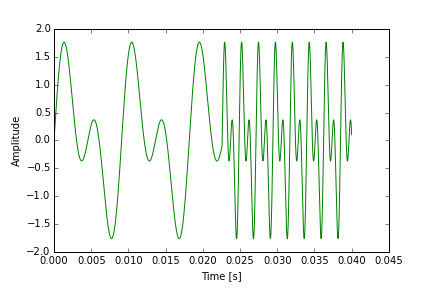
\includegraphics[width = \textwidth]{figures/sine_time_STFT.png}
		\caption{Two different tones represented in time.}
		\label{fig:sine_time_STFT}
	\end{subfigure}
	\begin{subfigure}{0.49\textwidth}
	\centering
		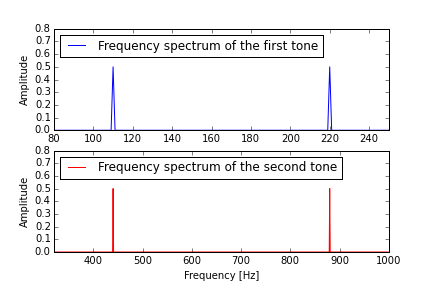
\includegraphics[width = \textwidth]{figures/sine_freq_STFT.png}
		\caption{Frequency spectrum of the tones.}
		\label{fig:sine_freq_STFT}
	\end{subfigure}
	\caption{Two tones represented in the time and frequency domain, respectively.}
	\label{fig:sine_STFT}
\end{figure}

Amazingly, the human ear and brain is able to perceive the bare signal $f$ and process it into a representation that provides simultaneous information about both time and frequency. This is actually what human beings call music and is represented through the staff system shown in figure \ref{fig:cmajor} in chapter \ref{ch2}. The goal of time-frequency analysis (at least in this project) is to imitate the ear and create a joint time-frequency representation of a signal \cite{page 22, FTFA}. This is the incentive for the short-time Fourier transform (STFT), which may be thought of as the mathematical analogue of the musical score \cite{page 37, FTFA}. The following is inspired by \cite{page 37, FTFA}.
\\ \\
The idea in the STFT is to obtain properties of a local frequency spectrum of $f$ by restricting it to an interval and taking the Fourier transform of this interval. $f$ is restricted on this interval by using a window function, which is close to 1 near the origin and decays towards zero at the edges, which is therefore a smooth cut-off function. The boundaries created by a sharp cut-off function will be interpreted by the Fourier transform as a discontinuity or an abrupt variation of the signal, which is obviously not desirable \cite{Davis}. The following definition defines the STFT.

\begin{definition}[The short-time Fourier transform]
Let $f,g \in \mathcal{L}^2(\mathbb{R}^d)$. For a fixed window function $g \neq 0$ the short-time Fourier transform of a function $f$ with respect to $g$ is defined as:
\begin{align}
V_gf(\tau,\omega) = \int_{\mathbb{R}^d} f(t) \overline{g(t - \tau)} e^{-2\pi j t \omega} dt \quad \textnormal{ for } \tau,\omega \in \mathbb{R}^d
\end{align}
\end{definition}

Figure (insert reference to the figure) illustrates how the window function slides along the $t$-axis as $x$ varies, which is why the STFT is often called the ``sliding window Fourier transform'' \martin{Indsæt figur, der illustrerer STFT'en. \textregistered}. Therefore, $V_g(\tau,\omega)$ can be thought of as a measure for the amplitude of the frequency band near $\omega$ at time $\tau$. The window function $g$ is usually kept fixed, and $V_gf$ is considered to be a linear mapping from functions on $\mathbb{R}^d$ to functions on $\mathbb{R}^{2d}$, which is known as the \textit{time-frequency plane} for $d=1$ in signal analysis \cite{page 38, FTFA}.
\\ \\
Clearly, the STFT depends on how wide the window is. Using a rather wide window leads to good \textit{frequency resolutions}, and e.g. constant frequencies are thus clearly visible in the time-frequency plane. However, a short pulse will be blurred in the time-frequency plane as a wide window can't exactly determine at what time the spike occurs. On the other hand, using a narrow window leads to good \textit{time resolutions}, which means that the spike is clearly visible at a given time, but constant frequencies are on the other hand blurred \cite{Davis}. This is due to the fact that it is fundamentally impossible to simultaneously have the complete information of a signal in both the time and frequency domain. This is a consequence of the Heisenberg uncertainty principle \cite{Wang}.

\subsection{The Heisenberg uncertainty principle}



- The discrete STFT? \\
- The Uncertainty Principle: page 26 and proof?